\documentclass[aspectratio=169,11pt]{beamer}
\usepackage{graphicx}
\usepackage{booktabs}
\usepackage{tikz}
\usetikzlibrary{arrows.meta,calc,decorations.pathreplacing}
\hypersetup{colorlinks=true,urlcolor=blue!70!black}

\setbeamertemplate{navigation symbols}{}
\setbeamertemplate{footline}[frame number]
\setbeamertemplate{itemize items}[circle]
\setbeamercolor{frametitle}{fg=black}
\setbeamercolor{title}{fg=black}
\setbeamercolor{structure}{fg=black!70}
\setbeamerfont{frametitle}{series=\bfseries}
\definecolor{accent}{RGB}{200,60,40}
\newcommand{\hl}[1]{\textcolor{accent}{#1}}
\newcommand{\credit}[1]{{\tiny\color{gray}#1}}

\title{Gaia}
\subtitle{Measuring the positions of two billion stars}
\author{SRMP 2026}
\date{Session 1}

\begin{document}

\begin{frame}
\titlepage
\end{frame}

%----------------------------------------------------------------------
\begin{frame}{A map of our galaxy}
\begin{columns}[c]
\column{0.42\textwidth}
\centering
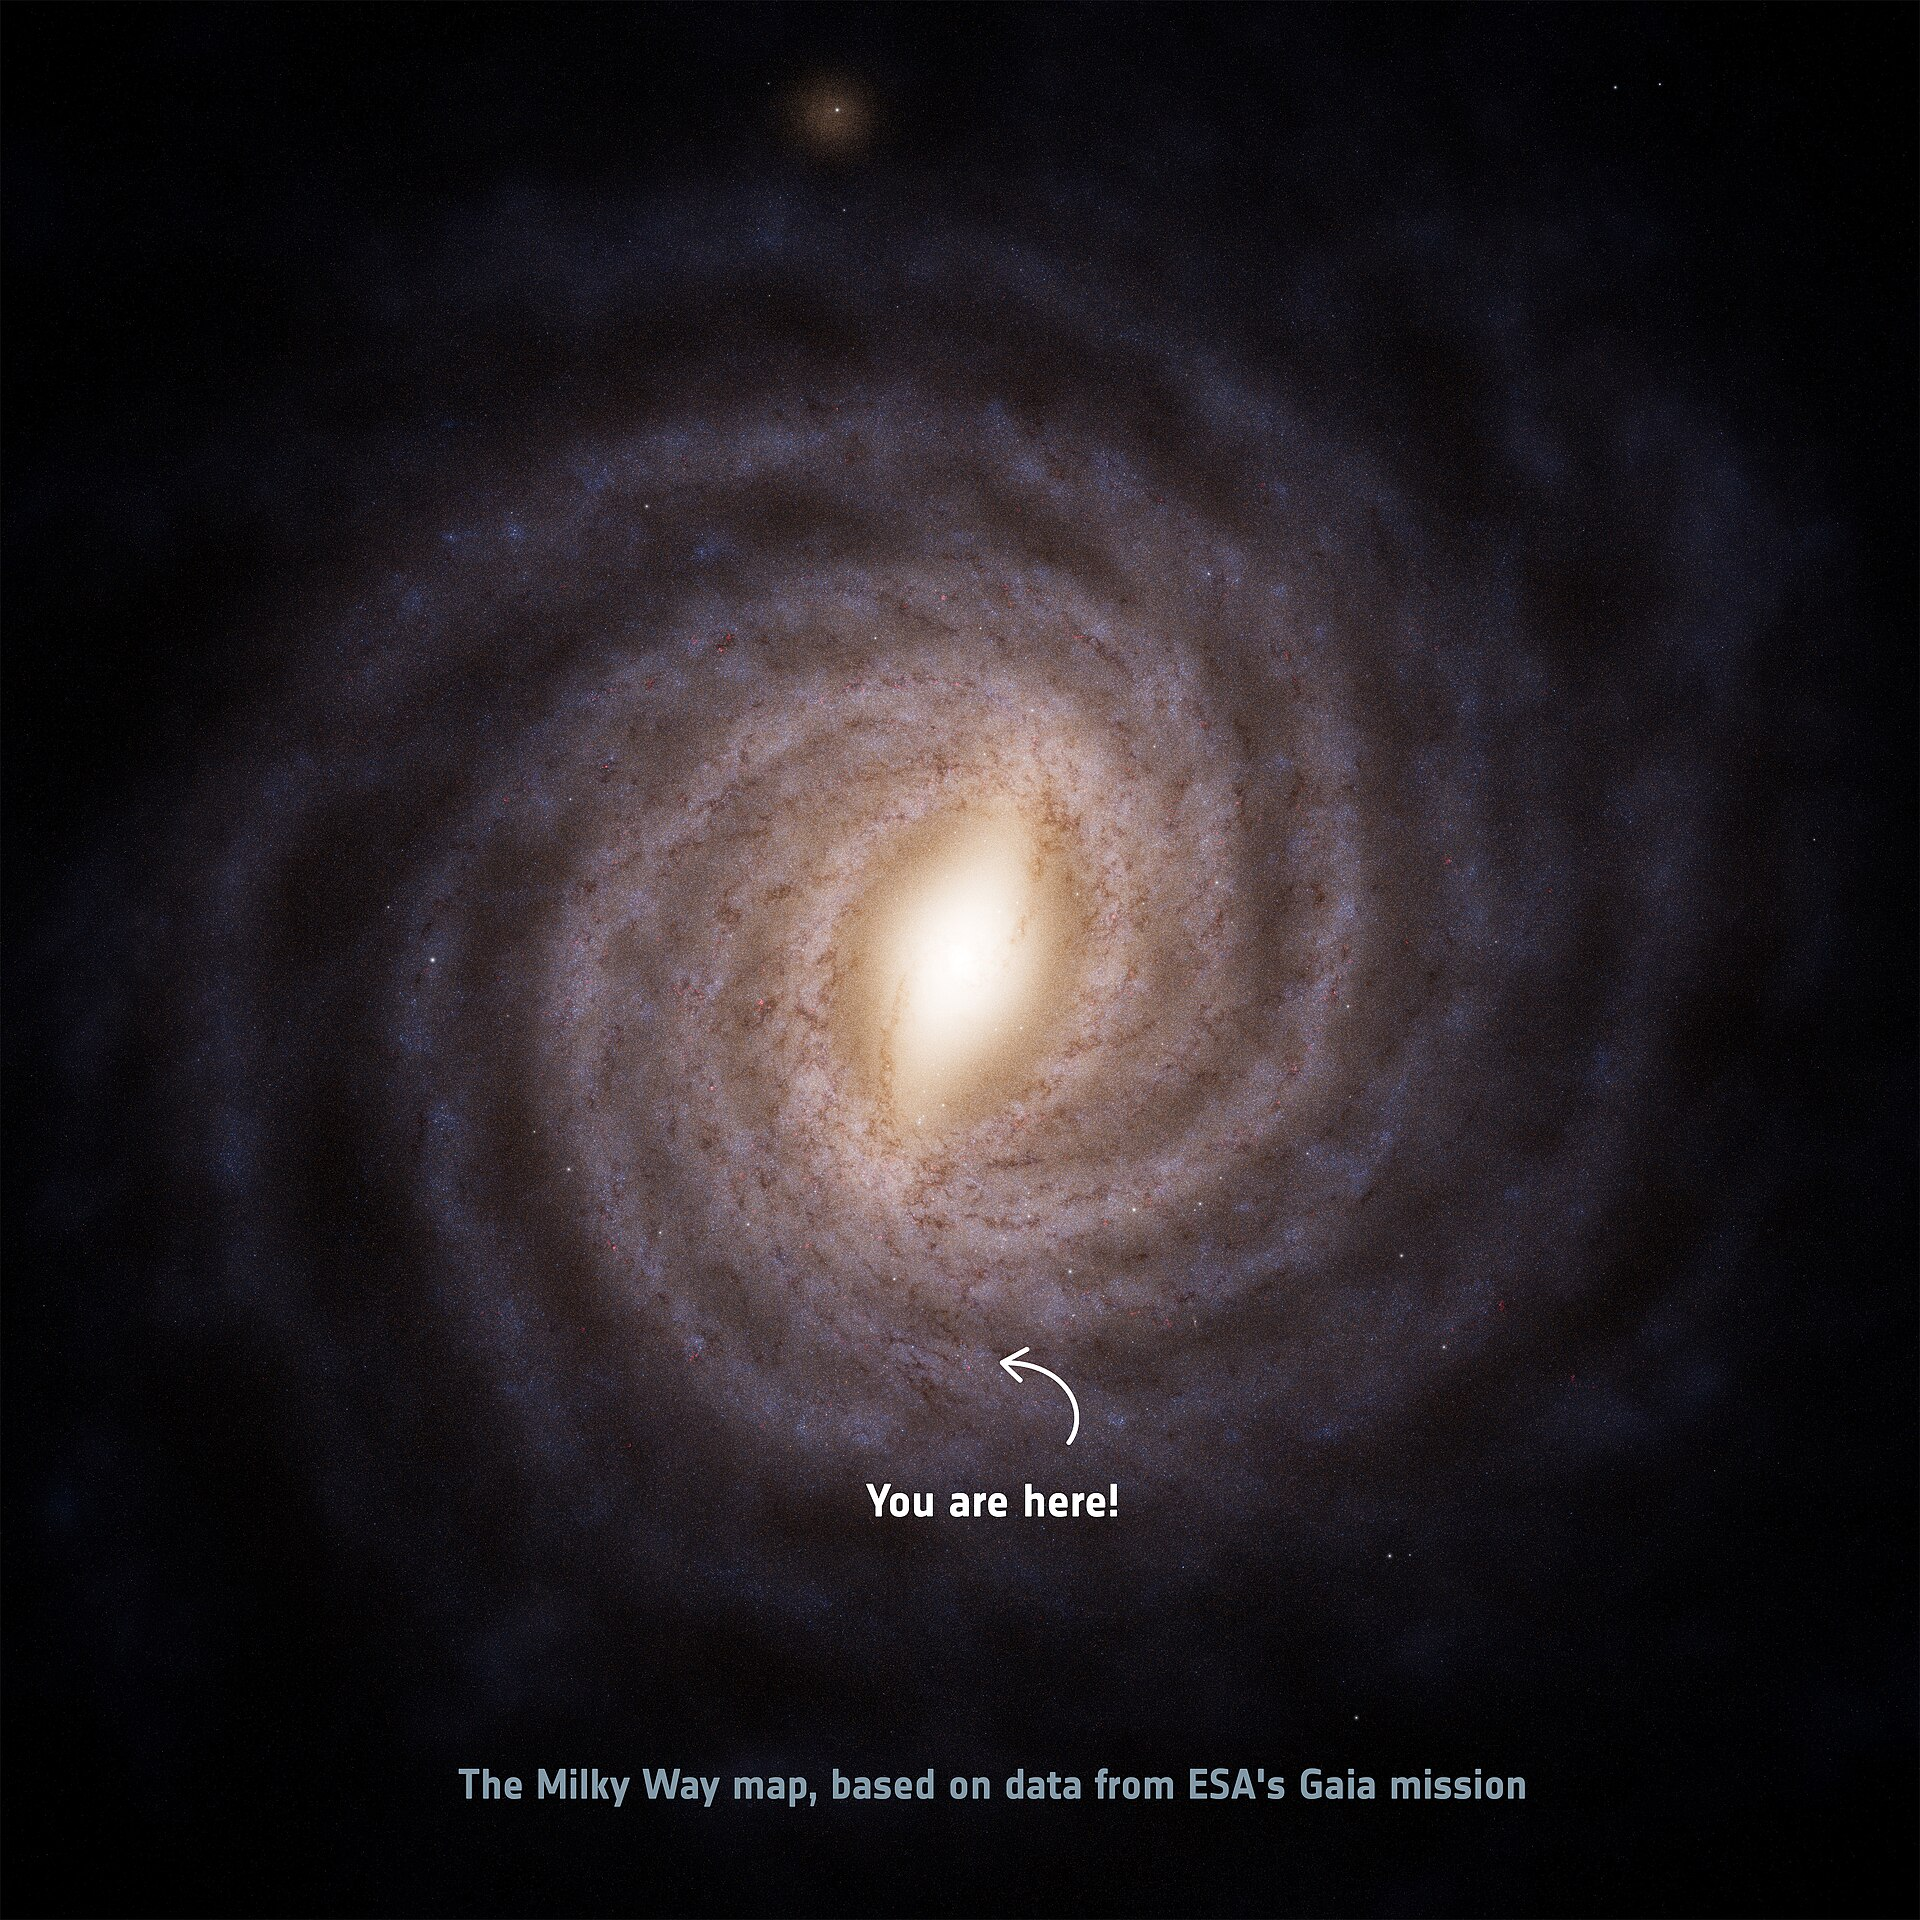
\includegraphics[height=0.78\textheight]{figures/images/milky_way_labelled.jpg}\\
\credit{ESA, CC BY-SA 3.0 IGO}
\column{0.58\textwidth}
\begin{itemize}
\item We live inside the Milky Way, so we can't step outside and take a picture of it.
\item Instead: measure where each star is and how it moves, then build the map.
\item Gaia measured positions for almost 2 billion stars, and distances and motions for 1.5 billion.
      That's about 1\% of the stars in our galaxy.
\item This picture is not a photo: it's an artist's drawing, based on Gaia's measurements.
\end{itemize}
\end{columns}
\end{frame}

%----------------------------------------------------------------------
\begin{frame}{How far away is a star? Parallax}
\begin{columns}[c]
\column{0.5\textwidth}
\begin{itemize}
\item Hold up a finger and blink one eye, then the other. Your finger jumps.
\item Same idea: look at a star in January, then in July. A nearby star seems to shift
      against the far-away ones.
\item The closer the star, the bigger the shift.
\end{itemize}
\vspace{0.5em}
\[ \text{distance [pc]} = \frac{1}{\text{parallax [arcsec]}} \]
\small 1 parsec (pc) = 3.26 light-years. An arcsec is a tiny angle (next slide).\\
Nearest star: parallax 0.77 arcsec, so distance = 1/0.77 = 1.3\,pc.
\column{0.5\textwidth}
\centering
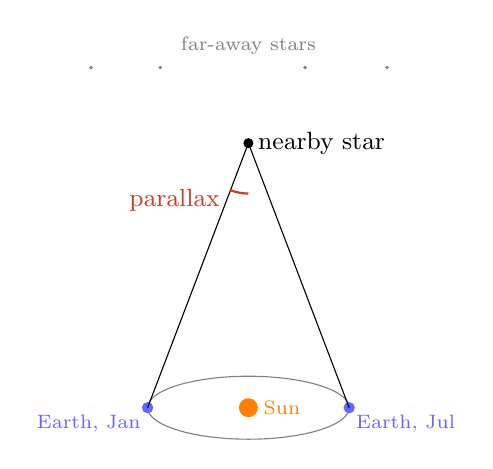
\begin{tikzpicture}[scale=0.8]
  \draw[gray] (0,0) ellipse (1.6 and 0.5);
  \fill[orange] (0,0) circle (0.15) node[right=2pt] {\scriptsize Sun};
  \fill[blue!60] (-1.6,0) circle (0.09) node[below left=-1pt] {\scriptsize Earth, Jan};
  \fill[blue!60] (1.6,0) circle (0.09) node[below right=-1pt] {\scriptsize Earth, Jul};
  \fill (0,4.2) circle (0.08) node[right] {\small nearby star};
  \draw[thin] (-1.6,0) -- (0,4.2) -- (1.6,0);
  \draw[accent,thick] (0,3.4) arc (-90:-111:0.8);
  \node[left,accent] at (-0.3,3.3) {\small parallax};
  \foreach \x in {-2.5,-1.4,0.9,2.2} \fill[gray] (\x,5.4) circle (0.03);
  \node[gray] at (0,5.75) {\scriptsize far-away stars};
\end{tikzpicture}
\end{columns}
\end{frame}

%----------------------------------------------------------------------
\begin{frame}{These angles are tiny}
1 arcsec (arcsecond) = 1/3600 of a degree.
\begin{center}
\begin{tabular}{lr}
\toprule
 & angle (arcsec) \\
\midrule
The full Moon & 1800 \\
Smallest detail your eye can see & 60 \\
Parallax of the nearest star & 0.77 \\
\hl{Gaia's precision, bright stars} & \hl{0.00002} \\
\bottomrule
\end{tabular}
\end{center}
\vspace{1em}
\begin{itemize}
\item 0.00002 arcsec is the width of a human hair seen from 1000\,km away
      (about Boston to Detroit).
\item Astronomers often use milliarcseconds: 1\,mas = 0.001 arcsec. So Gaia's best is 0.02\,mas.
\end{itemize}
\end{frame}

%----------------------------------------------------------------------
\begin{frame}{2000 years of measuring stars}
\begin{columns}[c]
\column{0.62\textwidth}
\centering
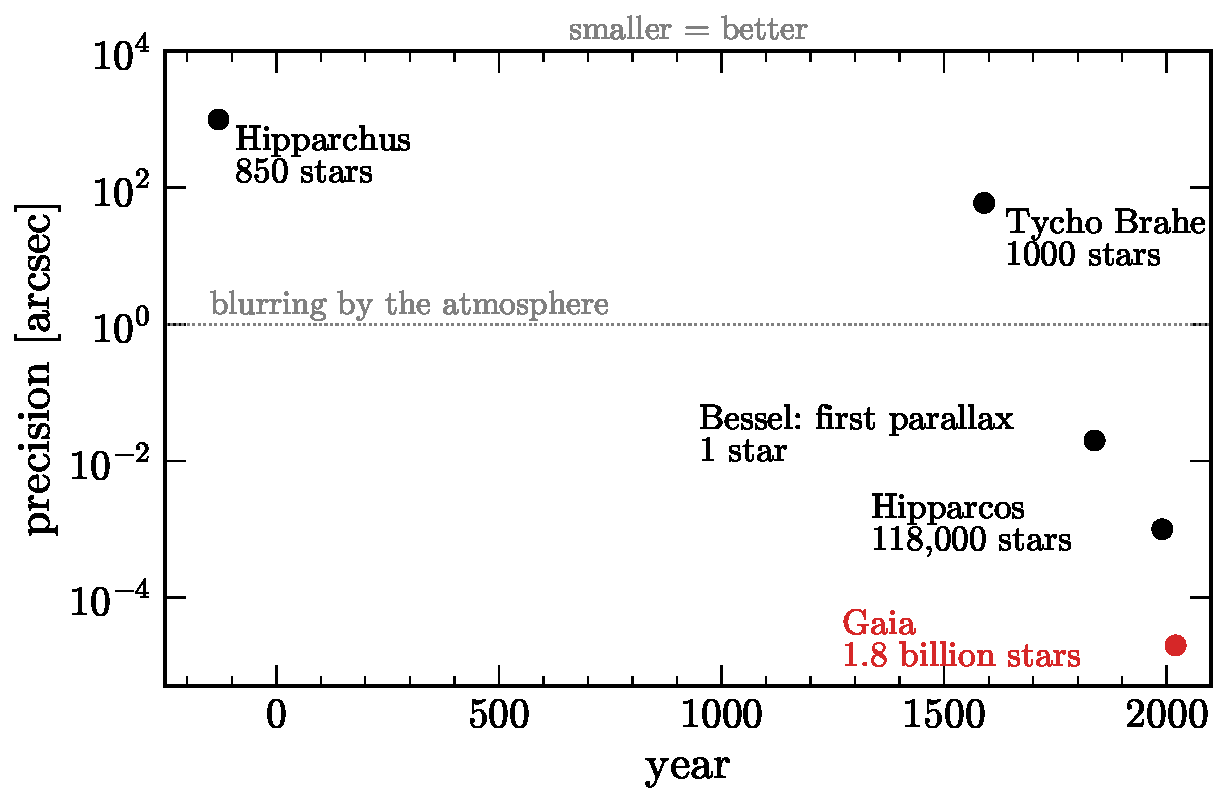
\includegraphics[width=\linewidth]{figures/history.pdf}
\column{0.38\textwidth}
\begin{itemize}
\item Each step down the left axis is 100 times smaller.
\item The atmosphere blurs stars to about 1 arcsec. Careful work from the ground beats that a little; space does far better.
\item Gaia: 50 times more precise than Hipparcos, for 15{,}000 times as many stars.
\end{itemize}
\end{columns}
\end{frame}

%----------------------------------------------------------------------
\begin{frame}{The spacecraft}
\begin{columns}[c]
\column{0.55\textwidth}
\centering
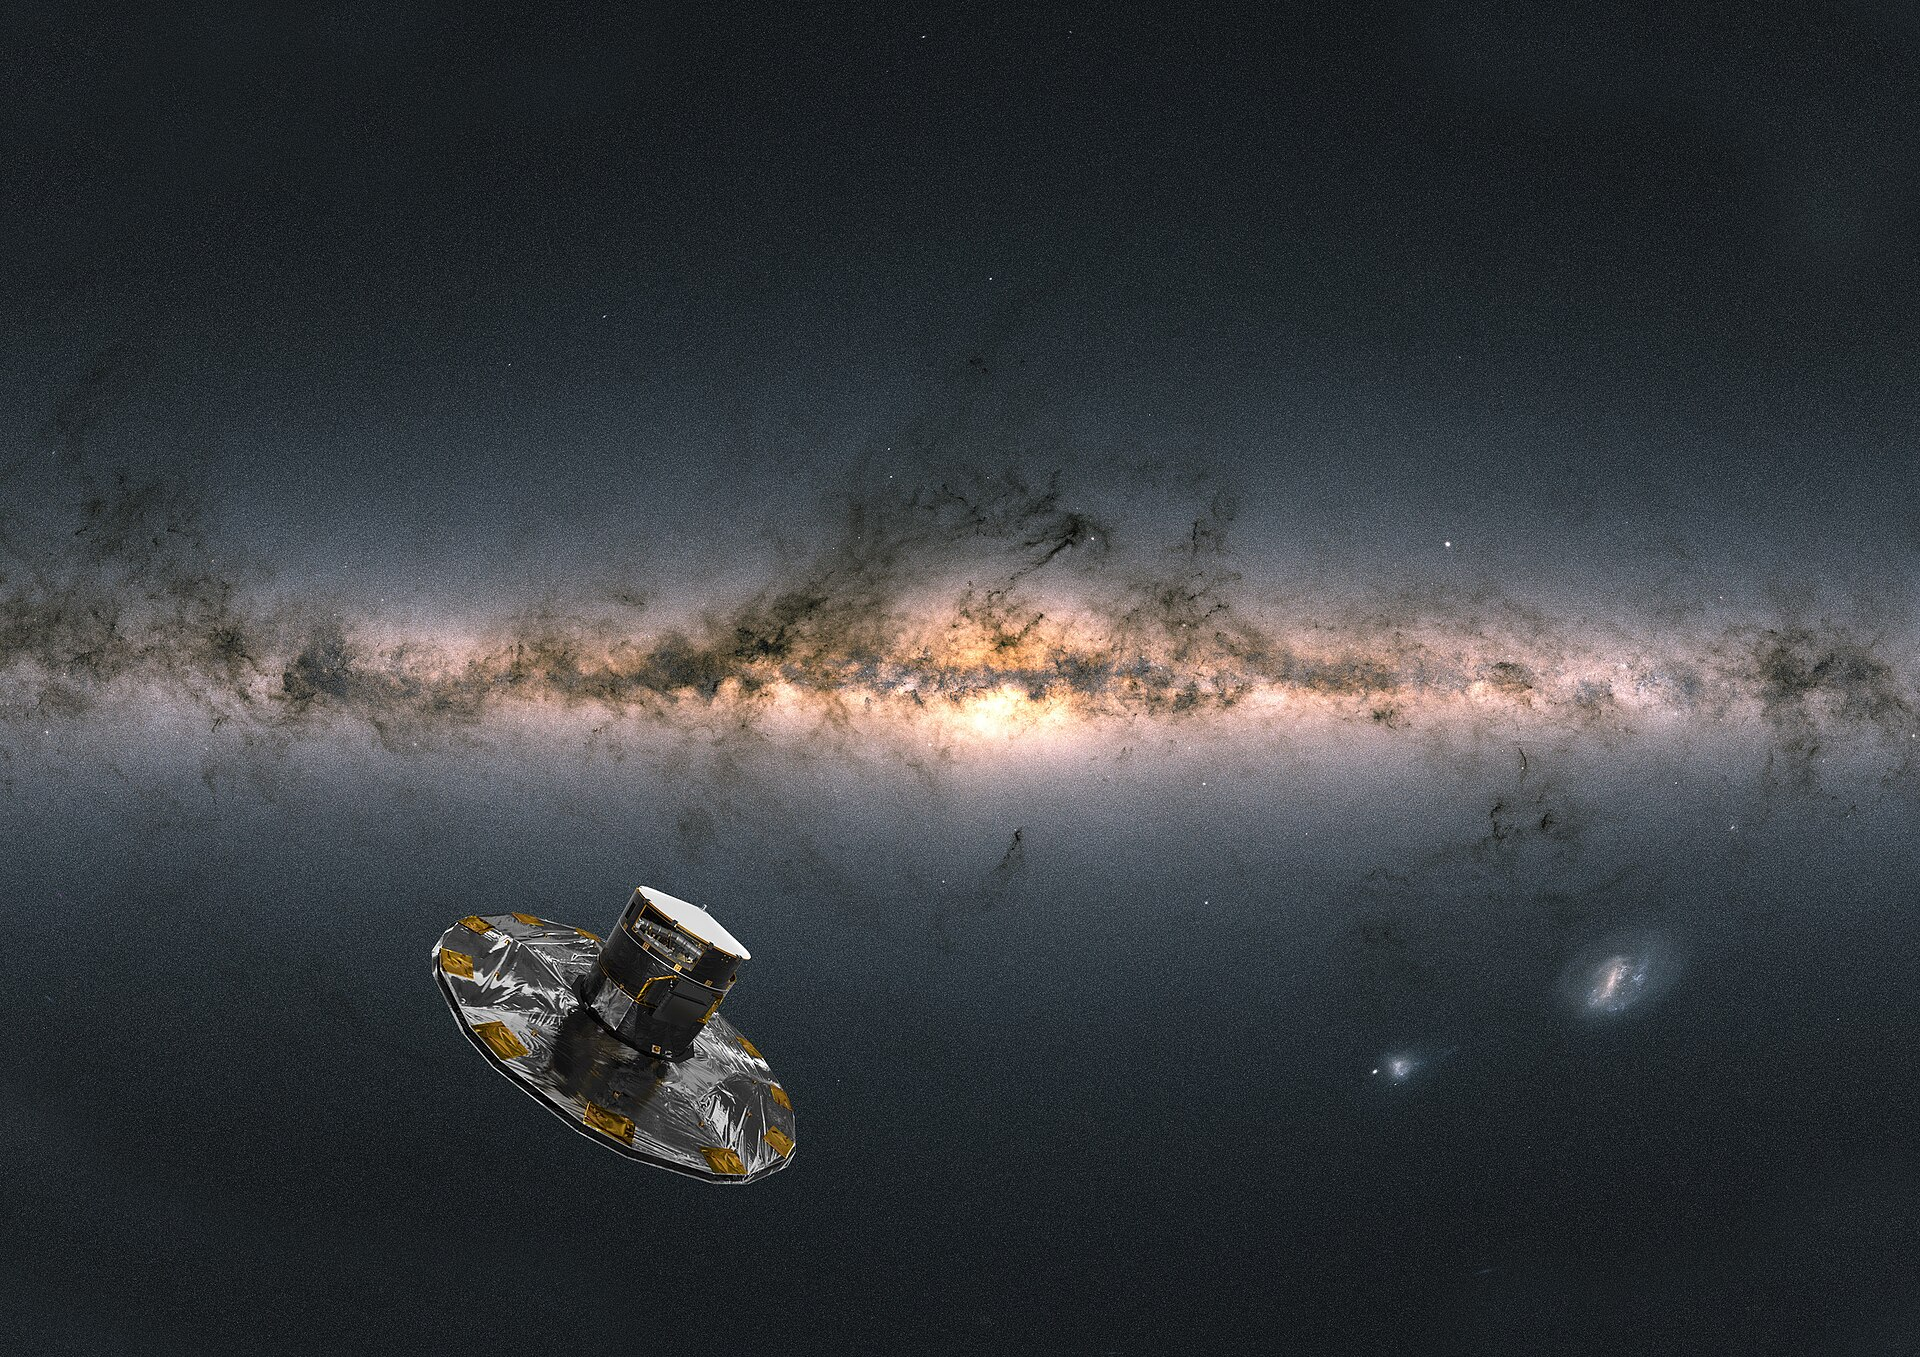
\includegraphics[width=\linewidth]{figures/images/gaia_spacecraft.jpg}\\
\credit{ESA, CC BY-SA 3.0 IGO}
\column{0.45\textwidth}
\begin{itemize}
\item Launched by the European Space Agency (ESA) in December 2013.
\item Sat 1.5 million km from Earth (4 times farther than the Moon), with the Sun, Earth and Moon all behind it.
\item Two telescopes, one giant camera: almost 1 billion pixels.
\item The 10\,m sunshield blocks the Sun, so the telescopes stay cold and steady.
\item Observed for 10.5 years, until January 2025.
\end{itemize}
\end{columns}
\end{frame}

%----------------------------------------------------------------------
\begin{frame}{How Gaia scanned the sky}
\begin{columns}[c]
\column{0.55\textwidth}
\centering
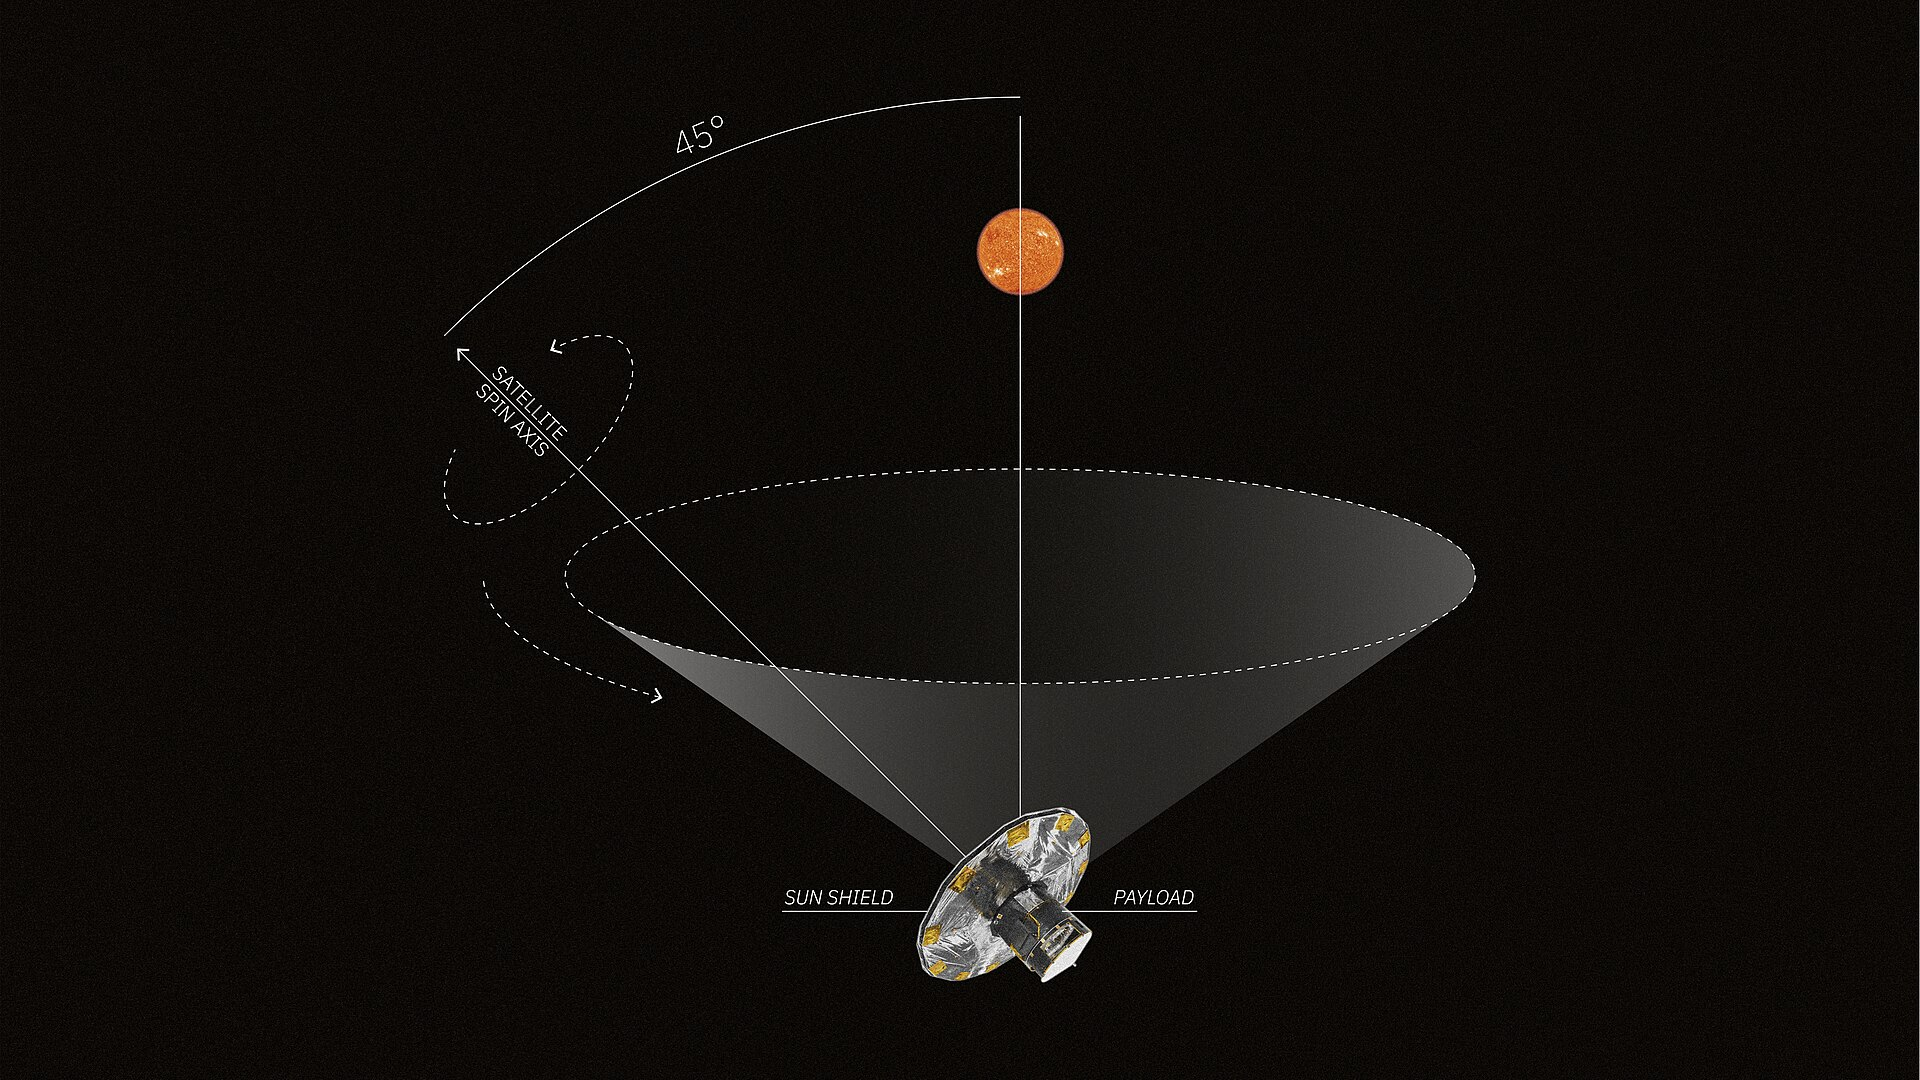
\includegraphics[width=\linewidth]{figures/images/gaia_rotation.jpg}\\
\credit{Space Travel Blog / R.\,M.\ Jansone / M.-L.\ Aru, CC BY 4.0}
\column{0.45\textwidth}
\begin{itemize}
\item Gaia spun slowly, once every 6 hours, sweeping its telescopes around a big circle on
      the sky.
\item The direction it spun around also slowly changed, so over months the circles covered the whole sky.
\item Over 10 years, each star was seen about 140 times.
\end{itemize}
\vspace{0.8em}
\textbf{Watch:} \href{https://www.youtube.com/watch?v=BnFyzZGWuYs}{Gaia scanning the sky}\\
{\scriptsize\href{https://www.youtube.com/watch?v=BnFyzZGWuYs}{youtube.com/watch?v=BnFyzZGWuYs}}
\end{columns}
\end{frame}

%----------------------------------------------------------------------
\begin{frame}{What Gaia measures}
\begin{columns}[T]
\column{0.33\textwidth}
\centering
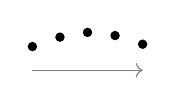
\begin{tikzpicture}
  \foreach \x/\y in {0/0,0.35/0.12,0.7/0.18,1.05/0.14,1.4/0.03} \fill (\x,\y) circle (0.06);
  \draw[->,gray] (0,-0.3) -- (1.4,-0.3);
\end{tikzpicture}\\[0.5em]
\textbf{Where}\\[0.3em]
\raggedright
Position on the sky, again and again.\\[0.3em]
$\rightarrow$ distance (parallax)\\
$\rightarrow$ how fast it moves across the sky
\column{0.33\textwidth}
\centering

\begin{tikzpicture}
  \fill[blue!60] (0,0) circle (0.2); \fill[orange!80] (0.7,0) circle (0.2); \fill[red!70] (1.4,0) circle (0.2);
\end{tikzpicture}\\[0.5em]
\textbf{Brightness and colour}\\[0.3em]
\raggedright
Through three filters: one wide, one blue, one red.\\[0.3em]
$\rightarrow$ how hot the star is\\
$\rightarrow$ whether it changes brightness
\column{0.33\textwidth}
\centering
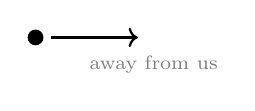
\begin{tikzpicture}
  \fill (0,0) circle (0.1);
  \draw[->,thick] (0.2,0) -- (1.3,0);
  \node[gray] at (1.5,-0.35) {\scriptsize away from us};
\end{tikzpicture}\\[0.5em]
\textbf{Speed toward or away}\\[0.3em]
\raggedright
By splitting its light into a rainbow, or spectrum (bright stars only).\\[0.3em]
$\rightarrow$ the third direction of motion
\end{columns}
\vspace{1.5em}
\centering
Together: a 3D map of the stars nearby, and how they move.
\end{frame}

%----------------------------------------------------------------------
\begin{frame}{The path of a star across the sky}
\centering
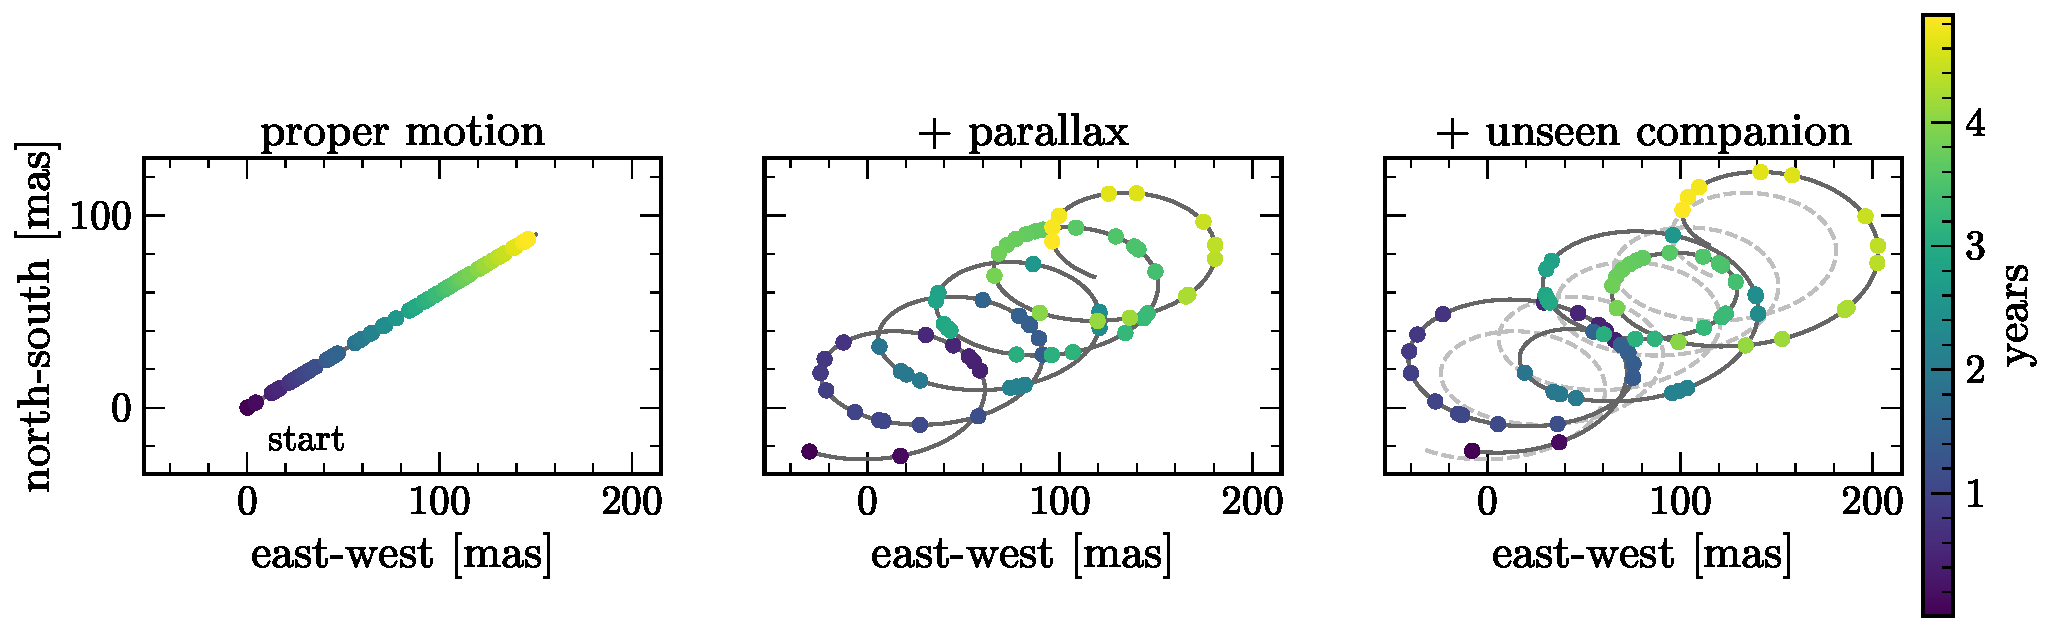
\includegraphics[width=0.95\textwidth]{figures/star_track.pdf}\\
\vspace{0.3em}
\small
A pretend star, seen 70 times over 5 years (colour = time). Left: it drifts in a straight line.
Middle: Earth's yearly trip around the Sun adds a loop (parallax). Right: an unseen companion adds
a wobble on top. The dashed line is the path without it. (The wobble is exaggerated.)
\end{frame}

%----------------------------------------------------------------------
\begin{frame}{How precise is it?}
\begin{columns}[c]
\column{0.5\textwidth}
\centering
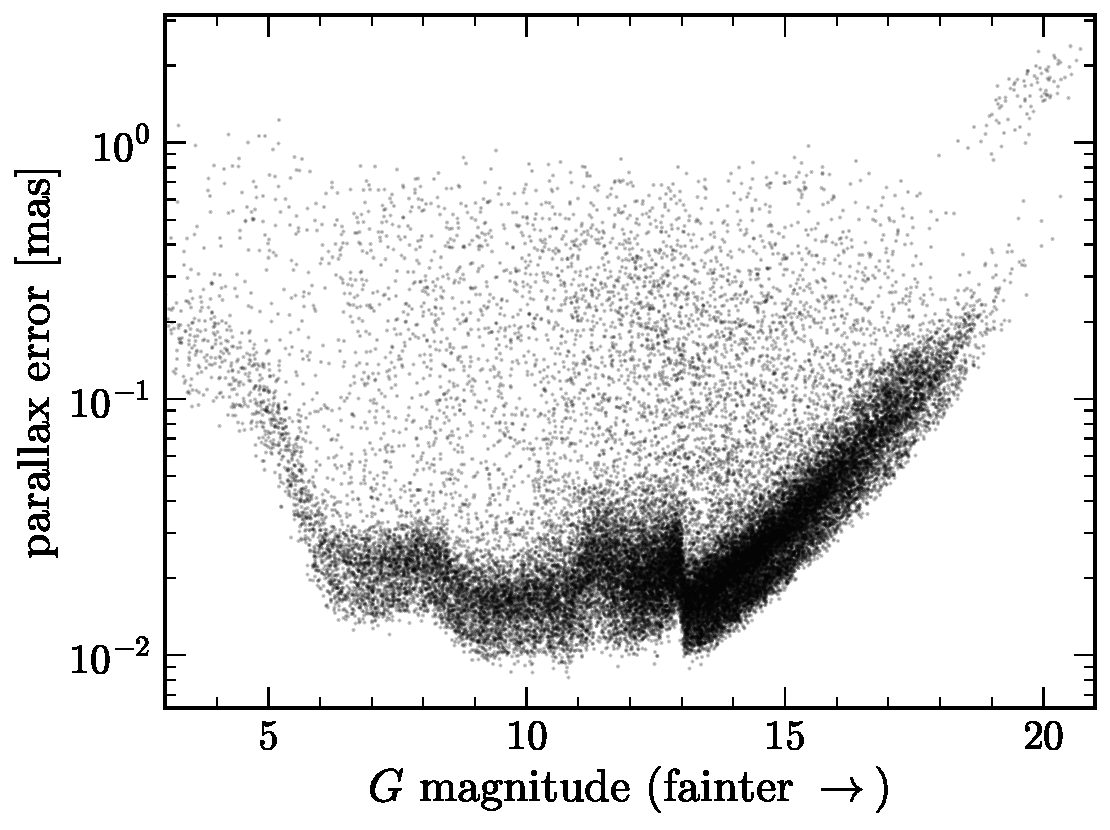
\includegraphics[width=\linewidth]{figures/plx_precision.pdf}
\column{0.5\textwidth}
\begin{itemize}
\item Each dot is a star within 50\,pc.
\item $G$ magnitude: how bright a star looks. It runs backwards: bigger number = fainter.
\item Fainter stars send less light, so their parallax is less certain.
\item The step at $G \approx 13$ comes from how the camera handles bright stars.
\end{itemize}
\end{columns}
\end{frame}

%----------------------------------------------------------------------
\begin{frame}{Data releases}
\centering
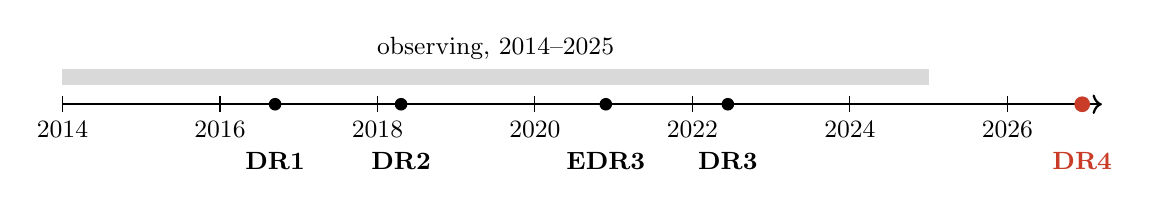
\begin{tikzpicture}[x=1.0cm]
  \draw[->,thick] (0,0) -- (13.2,0);
  \foreach \yr/\x in {2014/0,2016/2,2018/4,2020/6,2022/8,2024/10,2026/12} {
    \draw (\x,0.1) -- (\x,-0.1) node[below] {\small \yr};
  }
  \fill[gray!30] (0,0.25) rectangle (11,0.45);
  \node[above] at (5.5,0.45) {\small observing, 2014--2025};
  \foreach \x/\lab in {2.7/DR1,4.3/DR2,6.9/EDR3,8.45/DR3} {
    \fill (\x,0) circle (0.08);
    \node[below=14pt] at (\x,0) {\small\textbf{\lab}};
  }
  \fill[accent] (12.95,0) circle (0.1);
  \node[below=14pt,accent] at (12.95,0) {\small\textbf{DR4}};
\end{tikzpicture}
\vspace{1.5em}
\small DR = data release. EDR3 was the first half of DR3.
\begin{itemize}
\item \textbf{DR3} (2022): what we'll use in the tutorials. Average position, distance and motion
      for each star.
\item \textbf{DR4} (2 December 2026): 5.5 years of data, and \hl{every single measurement} of
      every star, not just averages.
\item \textbf{DR5} (around 2030): all 10.5 years.
\end{itemize}
\end{frame}

%----------------------------------------------------------------------
\begin{frame}{The whole sky, as seen by Gaia}
\centering
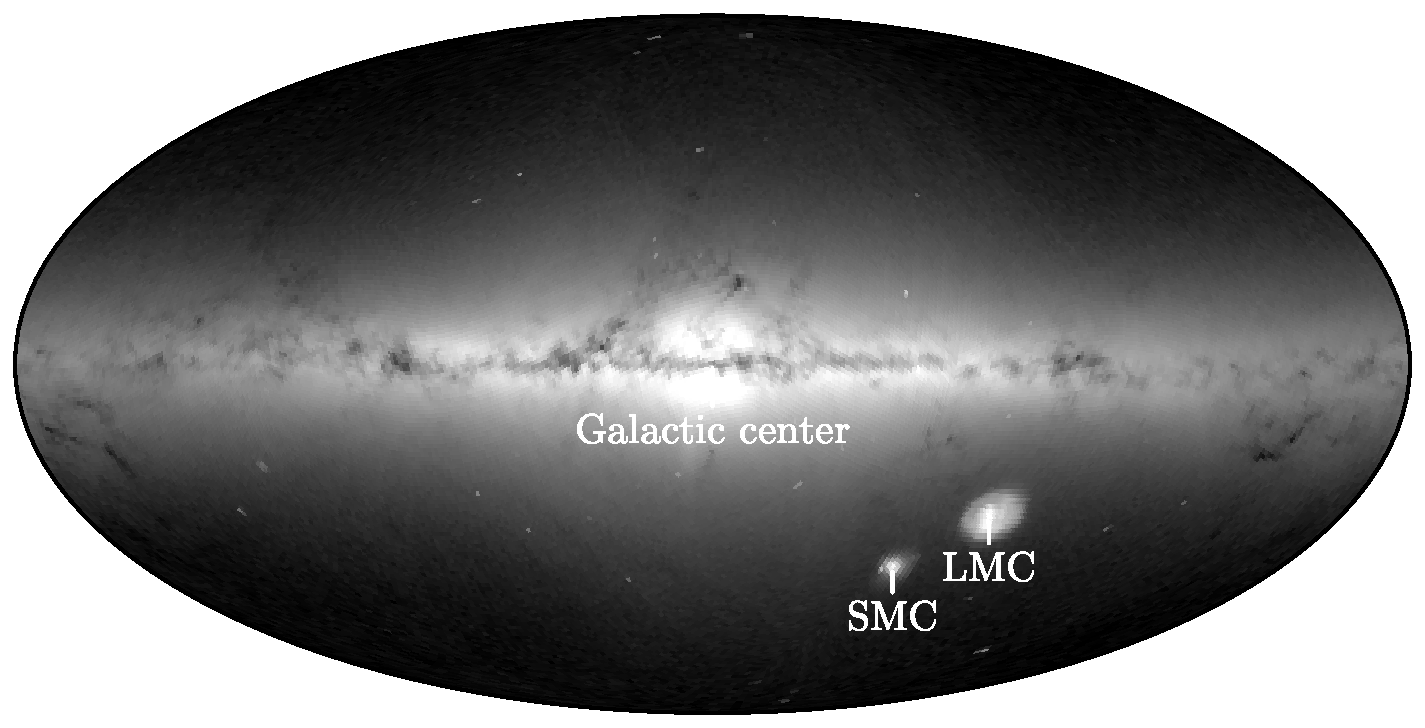
\includegraphics[width=0.8\textwidth]{figures/skymap.pdf}\\
\small
Number of stars per patch of sky in DR3. The whole sky is flattened into an oval, like a world map.
The Milky Way is a flat disk and we sit inside it, so it looks like a band across the middle. Dark
lanes are dust clouds. LMC and SMC are two small galaxies orbiting ours.
\end{frame}

%----------------------------------------------------------------------
\begin{frame}{Our neighbourhood: stars within 50\,pc}
\begin{columns}[c]
\column{0.45\textwidth}
\centering
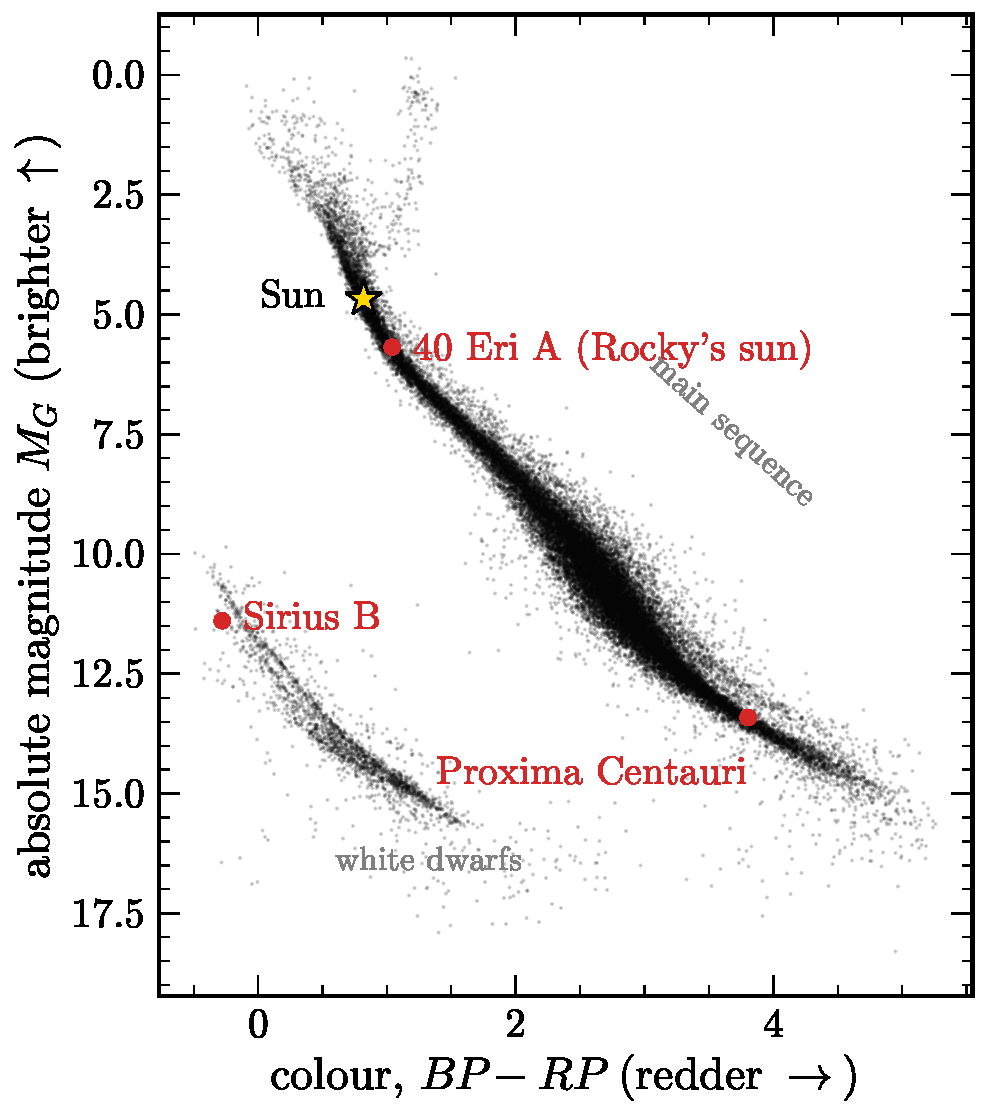
\includegraphics[height=0.82\textheight]{figures/hrd_50pc.pdf}
\column{0.55\textwidth}
\textbf{The Hertzsprung--Russell (HR) diagram}
\begin{itemize}
\item Left to right: hot blue stars to cool red stars.
\item Up: brighter. Using Gaia's distances, we work out how bright each star would look if
      they were all at the same distance (``absolute magnitude'').
\item Most stars sit on one band, the \hl{main sequence}. The Sun is one of them.
\item Bottom left: white dwarfs, the small, hot leftover cores of dead stars.
\item In \textit{Project Hail Mary}, Rocky's sun is a real star: 40 Eri A, 5\,pc away.
\end{itemize}
\end{columns}
\end{frame}

%----------------------------------------------------------------------
\begin{frame}[fragile]{Your turn: real Gaia data}
You'll download Gaia data yourself and remake the plots from today.
\vspace{0.5em}
\begin{block}{}
\small
\texttt{SELECT source\_id, ra, dec, parallax, phot\_g\_mean\_mag, bp\_rp}\\
\texttt{FROM gaiadr3.gaia\_source}\\
\texttt{WHERE parallax > 20}
\end{block}
\begin{itemize}
\item In words: ``For every star with parallax above 20\,mas (closer than 50\,pc), give me its
      ID, position on the sky (ra, dec), parallax, brightness and colour.''
\item The Gaia archive: \url{https://gea.esac.esa.int/archive/}
\end{itemize}
\end{frame}

%----------------------------------------------------------------------
\begin{frame}{References and image credits}
\footnotesize
\begin{itemize}
\item Gaia Collaboration, Prusti et al.\ 2016, \textit{The Gaia mission}, A\&A 595, A1
\item Gaia Collaboration, Vallenari et al.\ 2023, \textit{Gaia DR3: Summary of the content and
      survey properties}, A\&A 674, A1
\item Lindegren et al.\ 2021, \textit{Gaia EDR3: The astrometric solution}, A\&A 649, A2
\item ESA Gaia pages: \url{https://www.cosmos.esa.int/web/gaia}
\end{itemize}
\vspace{0.5em}
Images (via Wikimedia Commons):
\begin{itemize}
\item Milky Way map: ESA, CC BY-SA 3.0 IGO
\item Gaia spacecraft: ESA, CC BY-SA 3.0 IGO
\item Gaia scanning diagram: Space Travel Blog / R.\,M.\ Jansone / M.-L.\ Aru, CC BY 4.0
\end{itemize}
\vspace{0.5em}
Sky map, HR diagram and other plots made from Gaia DR3 data with the tutorial notebooks.
\end{frame}

\end{document}
